\documentclass[border=12pt]{standalone}
\usepackage{tikz}
\usepackage{amsmath}
\usetikzlibrary{positioning,arrows.meta,fit,backgrounds,calc}
\begin{document}
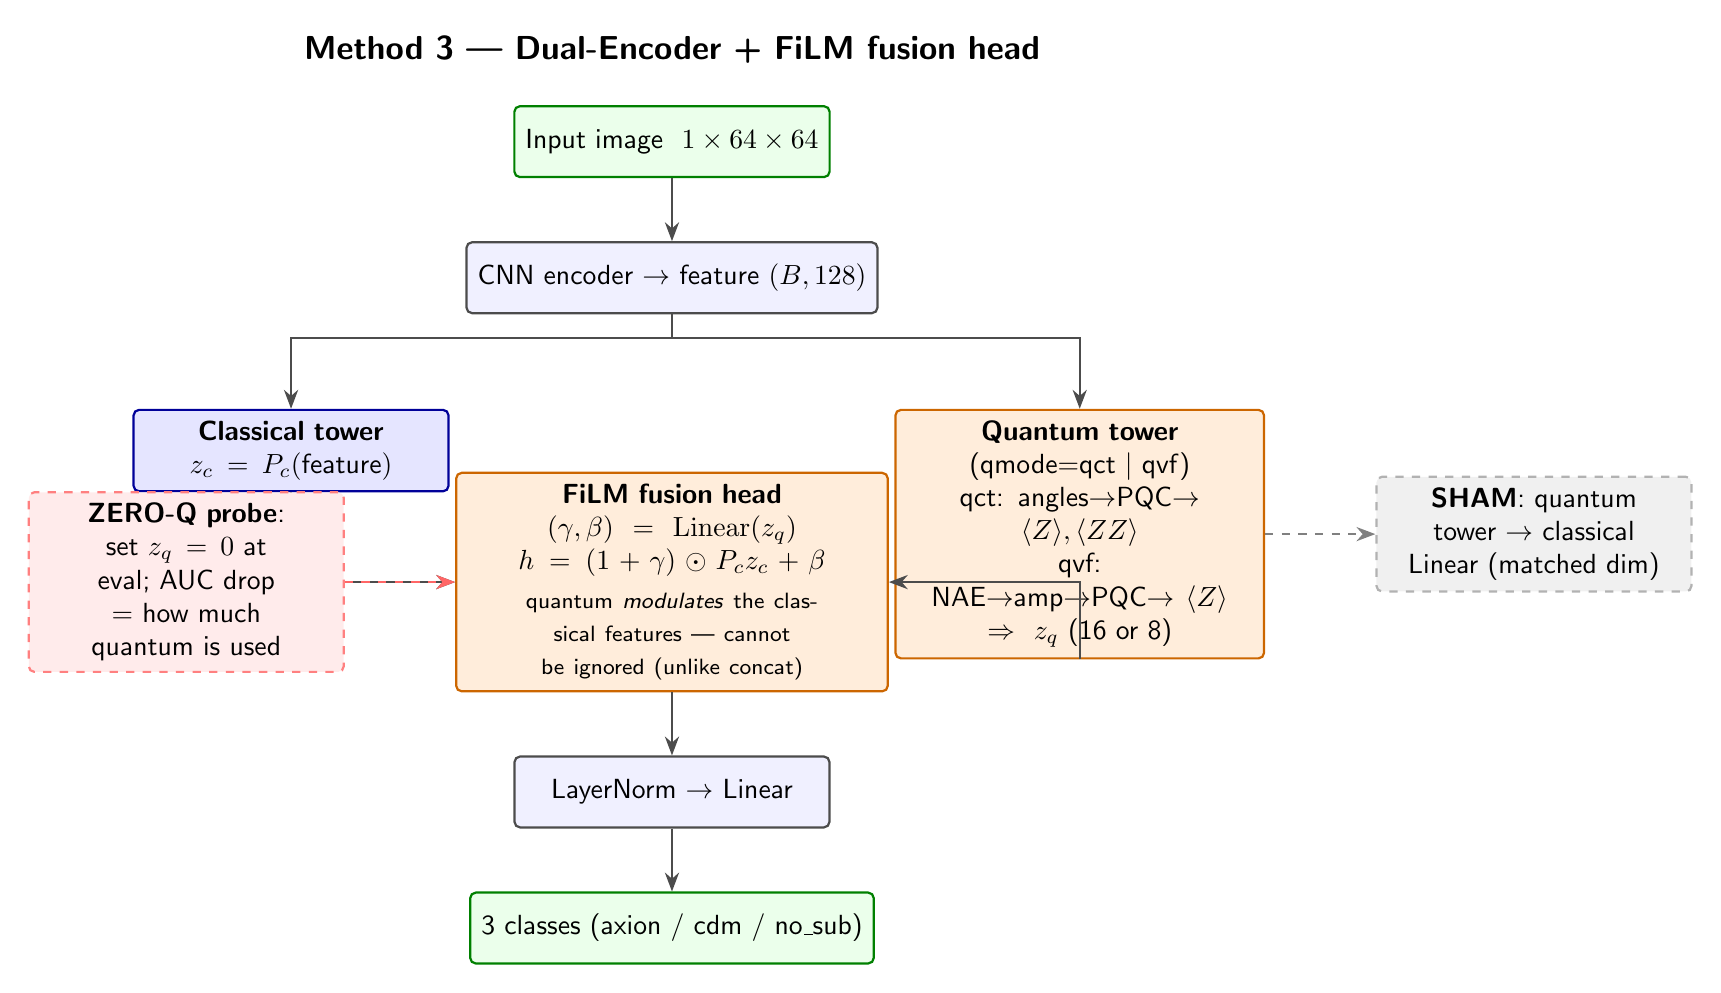
\begin{tikzpicture}[
  font=\sffamily,
  node distance=8mm,
  box/.style={rectangle,rounded corners=2pt,draw=black!70,thick,fill=blue!6,
              minimum height=9mm,minimum width=40mm,align=center,inner sep=4pt},
  qbox/.style={box,fill=orange!14,draw=orange!80!black},
  cbox/.style={box,fill=blue!10,draw=blue!60!black},
  shbox/.style={box,fill=gray!12,draw=gray!60,dashed},
  io/.style={box,fill=green!8,draw=green!50!black},
  arr/.style={-{Stealth[length=2.4mm]},thick,black!70},
]
\node[io] (img) {Input image \ $1\times64\times64$};
\node[box,below=of img] (cnn) {CNN encoder $\to$ feature $(B,128)$};

% two towers
\node[cbox,below left=12mm and 2mm of cnn,text width=36mm] (zc)
   {\textbf{Classical tower}\\$z_c = P_c(\text{feature})$};
\node[qbox,below right=12mm and 2mm of cnn,text width=44mm] (zq)
   {\textbf{Quantum tower} \ (qmode=qct $|$ qvf)\\
    qct: angles$\to$PQC$\to\langle Z\rangle,\langle ZZ\rangle$\\
    qvf: NAE$\to$amp$\to$PQC$\to\langle Z\rangle$\\
    $\Rightarrow z_q$ (16 or 8)};

\node[qbox,below=20mm of cnn,text width=52mm] (film)
   {\textbf{FiLM fusion head}\\
    $(\gamma,\beta)=\mathrm{Linear}(z_q)$\\
    $h=(1+\gamma)\odot P_c z_c+\beta$\\[2pt]
    \footnotesize quantum \emph{modulates} the classical
    features --- cannot be ignored (unlike concat)};
\node[box,below=of film] (head) {LayerNorm $\to$ Linear};
\node[io,below=of head] (out) {3 classes (axion / cdm / no\_sub)};

\draw[arr] (img)--(cnn);
\draw[arr] (cnn.south) -- ($(cnn.south)+(0,-3mm)$) -| (zc.north);
\draw[arr] (cnn.south) -- ($(cnn.south)+(0,-3mm)$) -| (zq.north);
\draw[arr] (zc.south) |- (film.west);
\draw[arr] (zq.south) |- (film.east);
\draw[arr] (film)--(head);
\draw[arr] (head)--(out);

\node[shbox,right=14mm of zq,text width=34mm] (sham)
   {\textbf{SHAM}: quantum tower $\to$ classical Linear (matched dim)};
\node[shbox,left=14mm of film,text width=30mm,fill=red!8,draw=red!50] (zero)
   {\textbf{ZERO-Q probe}: set $z_q=0$ at eval; AUC drop $=$ how much quantum is used};
\draw[arr,dashed,gray] (zq.east)--(sham.west);
\draw[arr,dashed,red!60] (zero.east)--(film.west);

\node[font=\sffamily\large\bfseries,above=4mm of img]
   {Method 3 — Dual-Encoder + FiLM fusion head};
\end{tikzpicture}
\end{document}
